 
\chapter{METODOLOGÍA}
Para poder cumplir todos los objetivos de la investigación, inicialmente se realizó la apropiación de 
conocimiento correspondiente con la temática y se definió el marco conceptual sobre el cual se iba a realizar el proyecto. Como primer paso 
fué importante entender la problemática que se pretende solucionar, identificar los recursos necesarios para el estudio y fijar las metas 
que se pretende alcanzar, las actividades mas relevantes empleadas en la investigación son detalladas a continuación:

\section{Identificar y Adquirir Imágenes Satelitales}
Se realiza el estudio de las imágenes satelitales más pertinentes para obtener la información, para la elección se tiene 
en cuenta 4 factores importantes \textit{resolución espacial}, \textit{resolución espectral}, \textit{resolución radiométrica} 
y \textit{resolución temporal} de la imágen satelital; Las imágenes de LandSat 7 son generadas cada 16 dias y permiten adquirir
datos de 8 bandas espectrales con una resolución de 15m por pixel para la banda 6 y 30m por pixel para las 7 bandas restantes, 
estas bandas tienen la capacidad de detectar diferentes indicadores para vegetación, reflectancia, temperatura, precipitación, 
nubosidad, etc. Por otra parte, las imágenes satelitales MODIS adquieren datos de 36 bandas espectrales con las cuales ofrece 
el producto MOD09GA con una resolución espacial aproximada de 500x500m en cada pixel, estos productos son generados diariamente 
y están diseñado para medir la reflectancia de la superficie terrestre\cite{mod09gadetails}\cite{modisweb}, MOD09GA 
presenta 7 banadas que tienen relación directa con la delimitación de territorios, tipos de vegetación, incidencia de aerosoles, 
temperatura y reflectancia la cual está relacionada con la propiedad reflectiva de la vegetación y los aerosoles; mediante la propiedad 
reflectiva de la vegetación se pretende realizar una estimación para la radiación solar que se irrádia en una superficie.



\textbf{Descarga de imágenes Satelitales}

Las imágenes satelitales de MODIS están ubicadas en una grilla senosoidal de aproximadamente 10x10 grados cada sección como lo muestra la 
figura~\ref{fig:gridmodis}. Esta grilla cuenta con un índice vertical y un índice horizontal que permiten ubicar la imagen satelital en un 
área determinada; el territorio colombiano se encuentra ubicado en la columna 10 (h10) en la fila 8 (v8) como lo muestra la 
figura~\ref{fig:colombiagridmodis}, estos 2 índices son necesarios para realizar la descarga de todas las imágenes satelitales comprendidas 
entre el año 2005 y 2015 para posteriormente construir la serie de tiempo de radiación solar. El gestor de descargas utilizado en esta 
ocasión es PyModis\cite{pymodisworkwithMODIS}, herramienta que permite la creación de scripts para gestionar las descargas, cambio de formato, 
procesamiento y reproyección de una imágen satelital a un sistema de coordenadas espaciales determinado.
\begin{figure}[htb]
  \centering 
  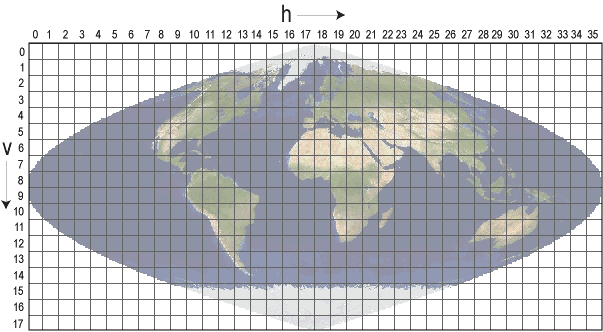
\includegraphics[scale=0.5]{pictures/MODIS_sinusoidal_grid.png}
  \caption{ Grilla Senosoidal de MODIS} 
  \label{fig:gridmodis}
\end{figure}

\begin{figure}[htb]
  \centering 
  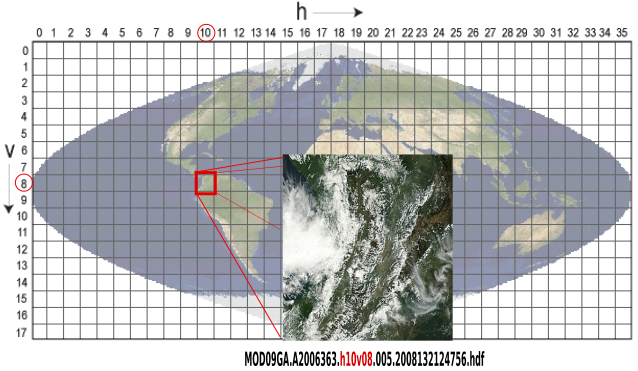
\includegraphics[scale=0.5]{pictures/mipc.png}
  \caption{ Ubicación del territorio colombiano en grilla senosoidal de MODIS} 
  \label{fig:colombiagridmodis}
\end{figure}
Para el caso del sensor MODIS el territorio colombiano y sus 32 departamentos se encuentra ubicado dentro de una sola imágen satelital, por este motivo 
solo se realizó la descarga diaria de una imágen durante los 11 años establecidos.

Por otra parte, las imágenes satelitales de LandSat 7 están ordenadas en una grilla de menor tamaño en comparación con la grilla de MODIS, para ubicar 
una imágen satelital en LandSat 7 se debe tener en cuenta PATH y ROW de las imágenes que logren la cobertura de una región definida como lo muestra 
la figura~\ref{fig:gridlandsat}, EarthExplorer\footnote{\url{http://earthexplorer.usgs.gov/}} permite identificar de manera sencilla las imágenes 
satelitales necesarias para la cobertura de un territorio.
\begin{figure}[htb]
  \centering 
  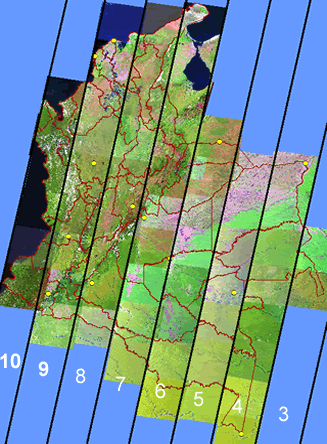
\includegraphics[scale=0.4]{pictures/pc.png}
  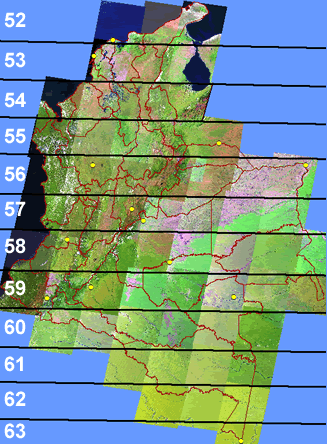
\includegraphics[scale=0.4]{pictures/rc.png}
  \caption{Path y Row de la Grilla sensor LandSat en Colombia - Fuente UNODC Colombia} 
  \label{fig:gridlandsat}
\end{figure}

Para el caso particular del departamento de Nariño, se logra una cobertura del territorio con 5 imágenes satelitales de LandSat 7 correspondientes a 
la lista de paths:rows (9:59), (9:60), (10:58), (10:59), (11:59) como lo muestra la figura~\ref{fig:nl7}.
\begin{figure}[htb]
  \centering 
  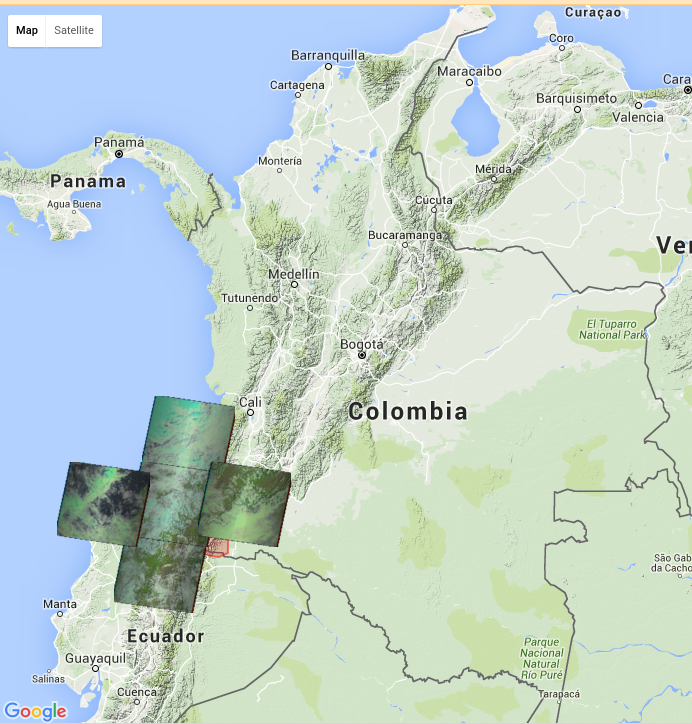
\includegraphics[scale=0.4]{pictures/nl7.png}
  \caption{Paths y Rows necesarios para la cobertura del territorio Nariñense.} 
  \label{fig:nl7}
\end{figure}

Actualmente existe software especializado en manejo de imágenes satelitales; gsutil\footnote{\url{https://cloud.google.com/storage/docs/gsutil}} 
dedicado explícitamente para la descarga de imágenes satelitales LandSat y pyModis\footnote{\url{http://pymodis.fem-environment.eu/}} que facilita 
la descarga y procesamiento a gran cantidad de imágenes satelitales proveniente del sensor MODIS. Para almacenar la información necesaria para 
la estimación de radiación solar sobre el departamento de Nariño se trabajó de forma independiente la manipulación de las imágenes LandSat y 
las imágenes de MODIS. 
\newpage
\section{Procesar y Almacenar Información}

Para el caso de MODIS se desarrolló un script dedicado al manejo de aproximadamente 3.500 imágenes satelitales MOD09GA, mediante el script se convierte 
el formato científico original de la imágen satelital(HDF) en un formato de imágenes de mapa de bits(TIFF) reproyectando el sistema de coordenadas 
espaciales original a  EPSG:3857, se utiliza EPSG:3857 por la simplicidad en cálculos, interpolación, aproximación y manejo en BD. Posterior a la conversión 
de formato y reproyección, se realizó un recorte a la imágen satelital en el que se abarque el territorio de Nariño y se proceda a recorrer las 7 bandas en 
formato TIFF obtenidas del producto MOD09GA, a continuación se almacenan muestras de reflectancia con referencia geográfica a cada 450 metros como lo muestra 
la figura~\ref{fig:dbmodis} y se aplíca el filtro de nubes según las especificaciones de las bandas\cite{bandMODISspecification}.
\begin{figure}[htb]
  \centering 
  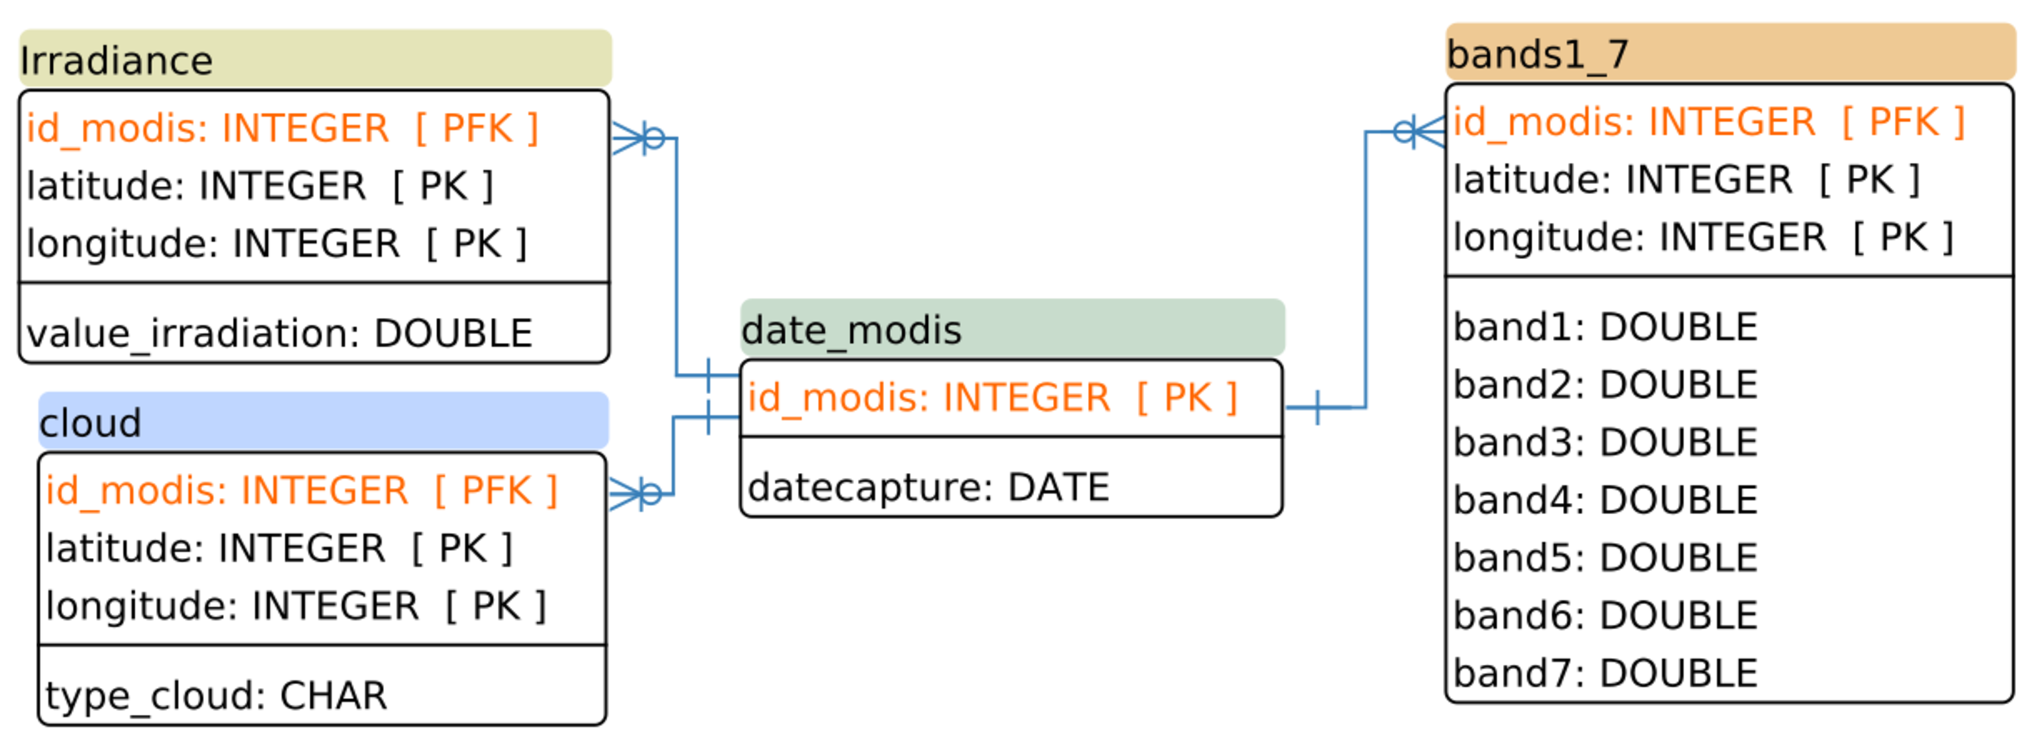
\includegraphics[scale=0.4]{pictures/bdmodis.pdf}
  \caption{Esquema BD para almacenamiento de imágenes satelitales MOD09GA.} 
  \label{fig:dbmodis}
\end{figure}
\newpage
Las imágenes provenientes del sensor LandSat 7 ofrecen 8 bandas que se encuentran compresas y en formato TIFF, para manipular este tipo de imágenes
se tiene en cuenta la reproyección del sistema de coordenadas espaciales original a  EPSG:3857 al igual que se lo realizo con las bandas de MOD09GA, 
para lograr la cobertura del departamento de Nariño es necesario la unión de 5 imágenes satelitales ver figura~\ref{fig:nl7u} y~\ref{fig:nl7}, luego se 
procede a realizar el recorte de la imagen satelital usando el croquis del departamento de Nariño ver figura~\ref{fig:nl7c}.
\begin{figure}[htb]
  \centering 
  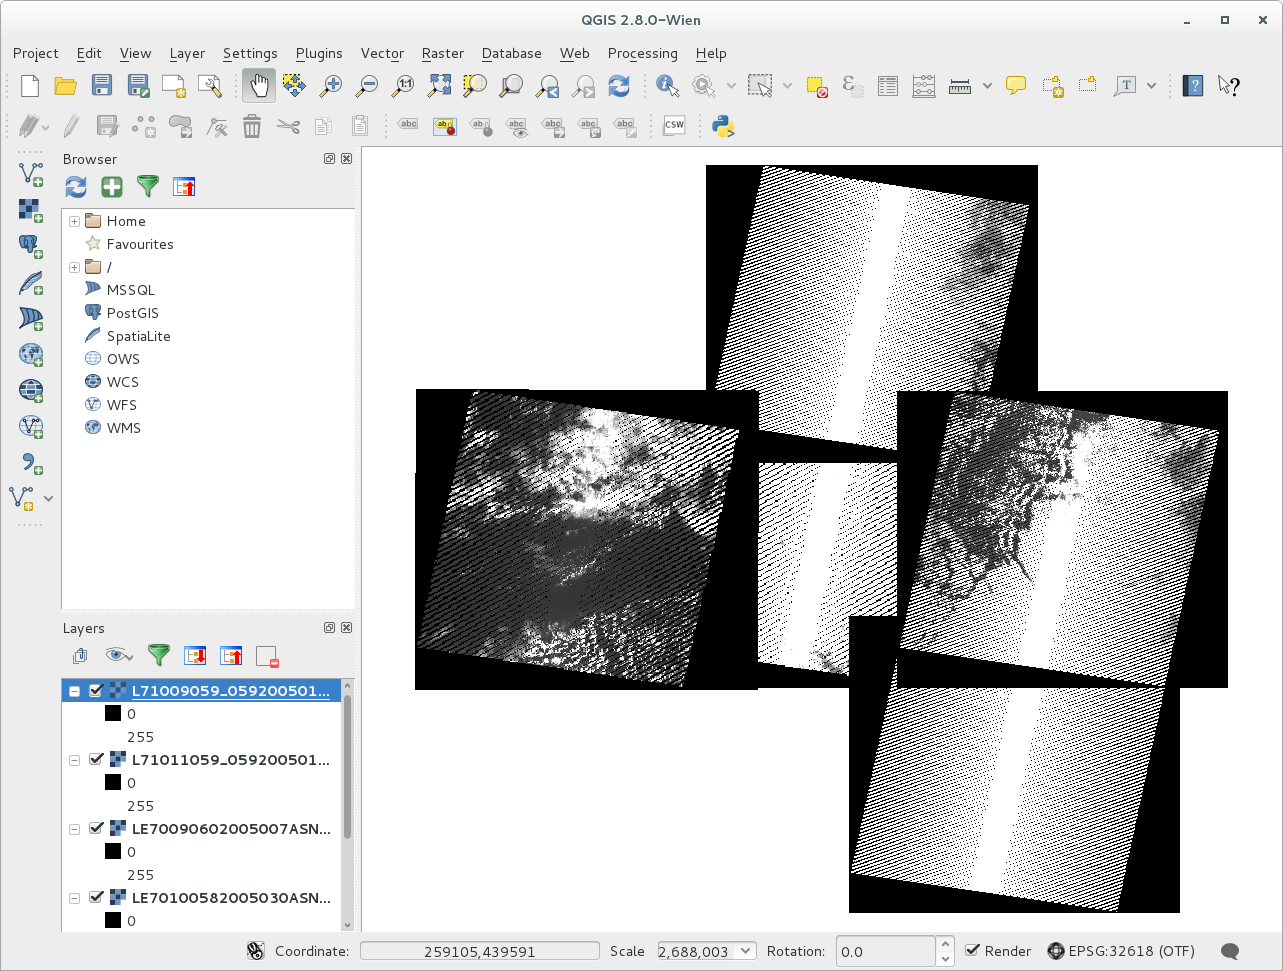
\includegraphics[scale=0.15]{pictures/cut1.png}
  \caption{Imágenes satelitales LandSat para lograr la cobertura del departamento de Nariño.} 
  \label{fig:nl7u}
\end{figure}
\begin{figure}[htb]
  \centering 
  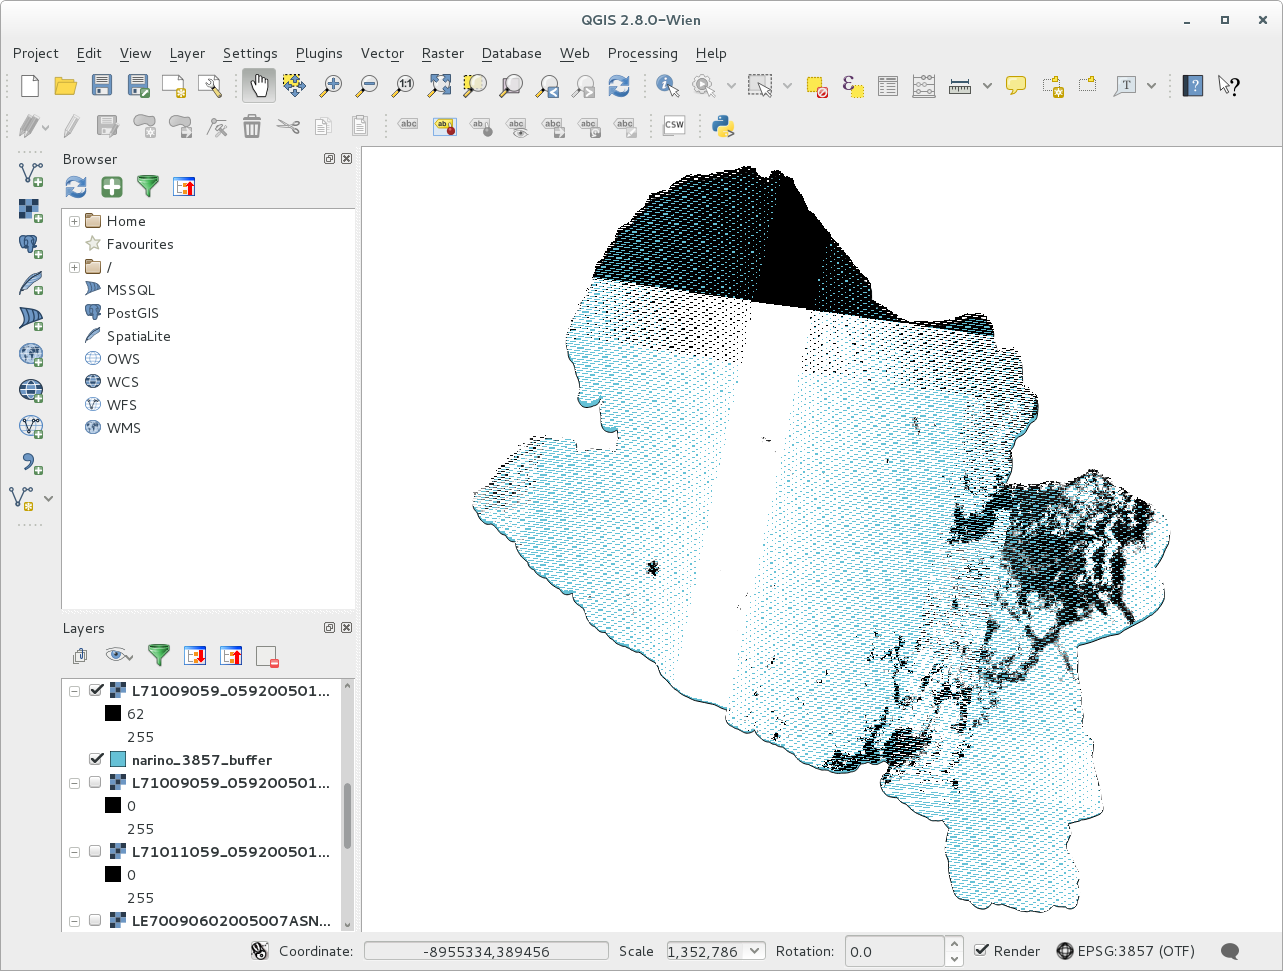
\includegraphics[scale=0.15]{pictures/cut2.png}
  \caption{Recorte de imágenes satelitales LandSat ajustado al territorio Nariñense.} 
  \label{fig:nl7c}
\end{figure}

Una vez terminado la reproyección y recorte de aproximadamente 1.300 imágenes satelitales, se procede a tomar muestras con referencia geográfica del Número 
Digital(DN) la imágen satelital, este número digital indica la escala de gris en la que se encuentra un pixel en determinada banda, esta escala de grises es 
interpretada de diferente forma en cada banda; una vez capturado el DN se procede a calcular la reflectancia, esto se realiza calibrando la muestra mediante 
correcciones atmosferica, estimación la ganancia de las bandas, corrección de ángulo de insidencia del sol, determinación de la distancia de la tierra al sol 
y calculos o correcciones recomendados por LandSat\cite{gasparri2007utilidad}.

La reflectancia obtenida es almacenada en BD ver figura~\ref{fig:dblansat} de igual forma se almacena información  de datos descartados al aplicar un filtro 
para detectar información de nubes, gases, lagos, ciudades, etc.\cite{cea2005mejoras}.
\begin{figure}[htb]
  \centering 
  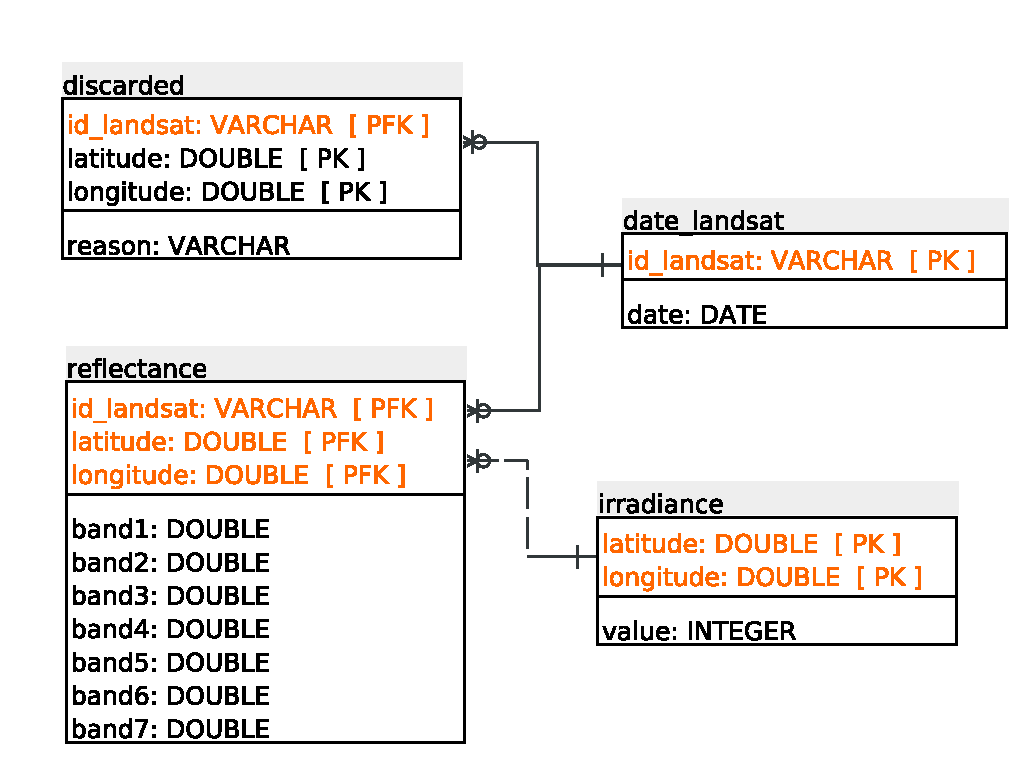
\includegraphics[scale=0.55]{pictures/landsatET.pdf}
  \caption{Esquema BD para almacenamiento de imágen satelital LandSat.} 
  \label{fig:dblansat}
\end{figure}

Finalizado el almacenamiento de las bandas presentes en la imágen satelital, se procede a realizar un muestreo de radiación solar georeferenciado 
proveniente de una fuente confiable de información, en este caso  se seleccionó 500 puntos distribuidos uniformemente sobre el territorio 
de Nariño y se procedió a consultar la información de 3TIER Figura~\ref{fig:m3t} para construir modelos de regresión y 
extrapolar los datos. Para la información referente a nubes se discrimino tres tipos de nubosidad correspondientes a la escala de 
reflectancia\cite{li2003high} según la altura del aerosol.
\begin{figure*}[htb]
  \centering
  \subfigure[Muestras Uniformemente distribuidas en el Departamento de Nariño]{\label{b1} 
  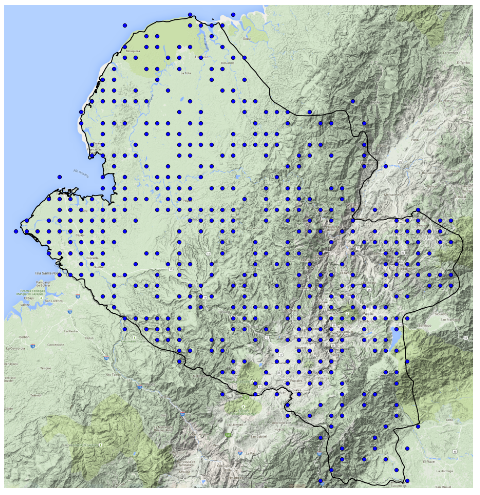
\includegraphics[scale=0.3]{pictures/m3tn.png}}\hspace{5mm}
  \subfigure[Muestras de radiación tomadas manualmente de 3TIER]{\label{b2} 
  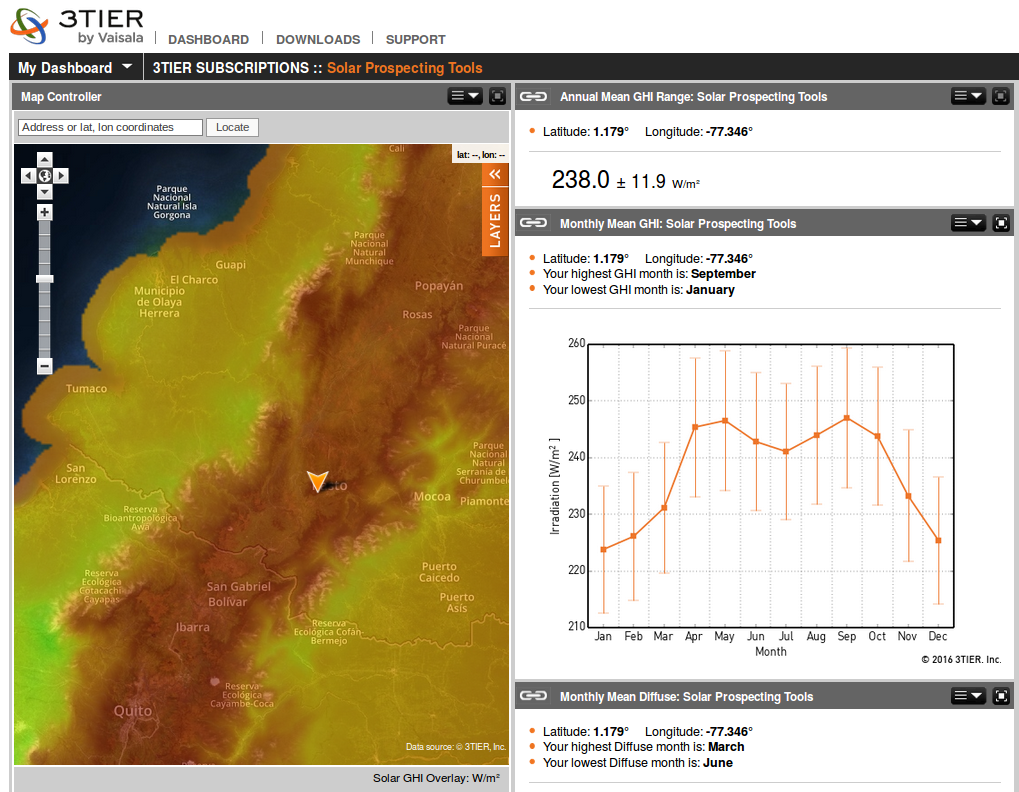
\includegraphics[scale=0.2]{pictures/3t.png}}
  \caption{Muestreo de radiación solar.}
  \label{fig:m3t}
\end{figure*}
\newpage

\section{Selección, Aplicación del Modelo de Regresión y Construcción de Serie de Tiempo}

En base a la información de las muestras recolectadas de 3TIER y la información recolectada de las bandas 1-7 del producto MOD09GA, se desarrolló un script en R 
para construir diferentes modelos de regresión, adicionalmente se evalúa cual es el modelo ideal para ser aplicado a la serie de tiempo y proceder a extrapolar 
los datos de reflectancia a datos de radiación solar, se realizó un análisis con 13 modelos para extrapolar los datos de reflectancia a datos de radiación.

Para la selección del modelo más adecuado se analizó las muestras de reflectancia del producto de MOD09GA y las muestras tomadas de 3TIER, mediante el 
análisis se obtuvo el resultado mostrado en la siguiente tabla ~\ref{tabla:arm}.
\begin{table}[H]
\centering\footnotesize
\begin{tabular}{ >{\arraybackslash}m{2cm} >{\arraybackslash}m{2cm} >{\arraybackslash}m{1.5cm} >{\arraybackslash}m{1.5cm} >{\arraybackslash}m{1.5cm} >{\arraybackslash}m{1.5cm} >{\arraybackslash}m{1.5cm}}
\hline
\textbf{Modelo}& \textbf{SAE} & \textbf{MAE} & \textbf{RAE} & \textbf{RMSE} & \textbf{COR} & $R^2$ \\
\hline \hline
ctree & 1360.88975 & 9.13349 & 60.07076 & 13.06545 & 0.64264 & 0.41299 \\
\hline
rpart & 1373.21922 & 9.21624 & 60.61499 & 14.14182 & 0.60074 & 0.36089 \\
\hline
kknn & 920.48535 & 6.17775 & 40.63096 & 10.31934 & 0.79280 & 0.62854 \\
\hline
mlp & 485.60361 & 3.25908 & 21.43493 & 4.51435 & 0.96284 & 0.92705 \\
\hline
\textbf{mlpe} & \textbf{443.11836} & \textbf{2.97395} & \textbf{19.55960} & \textbf{3.97730} & \textbf{0.97157} & \textbf{0.94394} \\
\hline
ksvm & 823.63424 & 5.52775 & 36.35587 & 8.12712 & 0.87861 & 0.77195 \\
\hline
randomForest & 1159.07988 & 7.77906 & 51.16271 & 11.04659 & 0.75129 & 0.56444 \\
\hline
mr & 597.58282 & 4.01062 & 26.37778 & 5.36391 & 0.94694 & 0.89670 \\
\hline
mars & 618.82261 & 4.15317 & 27.31532 & 5.47634 & 0.94475 & 0.89255  \\
\hline
cubist & 597.29188 & 4.00867 & 26.36494 & 5.36508 & 0.94688 & 0.89658 \\
\hline
pcr & 597.58282 & 4.01062 & 26.37778 & 5.36391 & 0.94694 & 0.89670 \\
\hline
plsr & 597.58282 & 4.01062 & 26.37778 & 5.36391 & 0.94694 & 0.89670 \\
\hline
cppls & 597.58282 & 4.01062 & 26.37778 & 5.36391 & 0.94694 & 0.89670 \\
\hline
\end{tabular}
\caption{\scriptsize{Análisis de modelos de Regresión aplicados a datos de reflectancia de 7 bandas de MOD09GA.}}
\label{tabla:arm}
\end{table}

Para encontrar el modelo más adecuado se realizó un análisis a los datos de reflectancia de LandSat y las muestras tomadas de 3TIER, los resultados se observan 
en la siguiente tabla~\ref{tabla:arl}.
\begin{table}[H]
\centering\footnotesize
\begin{tabular}{ >{\arraybackslash}m{2cm} >{\arraybackslash}m{2cm} >{\arraybackslash}m{1.5cm} >{\arraybackslash}m{1.5cm} >{\arraybackslash}m{1.5cm} >{\arraybackslash}m{1.5cm} >{\arraybackslash}m{1.5cm}}
\hline
\textbf{Modelo}& \textbf{SAE} & \textbf{MAE} & \textbf{RAE} & \textbf{RMSE} & \textbf{COR} & $R^2$ \\
\hline \hline
ctree & 771.66185 & 5.32181 & 33.37397 & 8.89544 & 0.85991 & 0.73945 \\
\hline
rpart & 819.97501 & 5.65500 & 35.46349 & 9.23174 & 0.84774 & 0.71865 \\
\hline
kknn & 583.36151 & 4.02318 & 25.23008 & 6.19161 & 0.93584 & 0.87580 \\
\hline
mlp & 558.43603 & 3.85128 & 24.15206 & 5.49114 & 0.94968 & 0.90189 \\
\hline
\textbf{mlpe} & \textbf{461.93253} & \textbf{3.18574} & \textbf{19.97834} & \textbf{4.73616} & \textbf{0.96292} & \textbf{0.92721} \\
\hline
ksvm & 574.76656 & 3.96391 & 24.85835 & 5.71528 & 0.94664 & 0.89613 \\
\hline
randomForest & 663.70528 & 4.57728 & 28.70490 & 6.89480 & 0.92117 & 0.84856 \\
\hline
mr & 752.19550 & 5.18756 & 32.53206 & 6.75745 & 0.92222 & 0.85049 \\
\hline
mars & 680.67053 & 4.69428 & 29.43864 & 6.34212 & 0.93186 & 0.86837 \\
\hline
cubist & 538.20590 & 3.71176 & 23.27712 & 6.34056 & 0.93141 & 0.86752 \\
\hline
pcr & 748.89239 & 5.16478 & 32.38920 & 6.76538 & 0.92208 & 0.85023 \\
\hline
plsr & 748.89239 & 5.16478 & 32.38920 & 6.76538 & 0.92208 & 0.85023 \\
\hline
cppls & 748.89239 & 5.16478 & 32.38920 & 6.76538 & 0.92208 & 0.85023 \\
\hline
\end{tabular}
\caption{\scriptsize{Análisis de modelos de Regresión aplicados a datos de reflectancia de 8 bandas de LandSat.}}
\label{tabla:arl}
\end{table}

%Las metricas evaluadas indican 
%\scriptsize{
%\texttt{\noindent
%\hspace{7ex}$R^2\to $Coeficiente de determinación\\
%\phantom{x}\hspace{6ex}$COR\to $Correlación\\
%\phantom{x}\hspace{6ex}$RMSE\to $Raíz del error cuadrático medio\\
%\phantom{x}\hspace{6ex}$RAE\to $Error absoluto relativo\\
%\phantom{x}\hspace{6ex}$MAE\to $Error medio absoluto\\
%\phantom{x}\hspace{6ex}$RMSE\to $Raíz del error cuadrático medio\\
%\phantom{x}\hspace{6ex}$SAE\to $Suma (Error Absoluto)/(Desviacion)\\
%}}
Según las métricas SAE, MAE, RAE, RMSE, COR y $R^2$ evaluadas en los 13 modelos \cite{ASH:2013:Online}, se logra concluir que el modelo más óptimo para extrapolar 
los datos de radiación es ``mlpe''–multilayer perceptron ensemble, mlpe es un modelo implementado en R que se basa en una red neuronal artificial con la capacidad 
de detectar características en los datos de la bandas de las imágenes satelitales LandSat y el producto MOD09GA, posteriormente el modelo se encarga de asociarlos 
a un valor objetivo y determinar las métricas de relación más comunes. Al realizar el análisis de los modelos se logra construir los todos modelos de regresión que 
son utilizados para extrapolar los datos, en este caso se procede a construir la serie de tiempo de radiación solar mediante la aplicación del modelo más óptimo; 
mlpe se encarga de evaluar los datos de reflectancia contenidos en las 7 bandas de MOD09GA y asocia un resultado de radiación que es almacenado en BD, de la misma 
forma analiza las 8 bandas de LandSat almacenados en la relación Radiance de la BD ver figura~\ref{fig:mlpe} y entrega como resultado un valor de radiación que es 
almacenado en BD.

\begin{figure}[htb]
  \centering 
  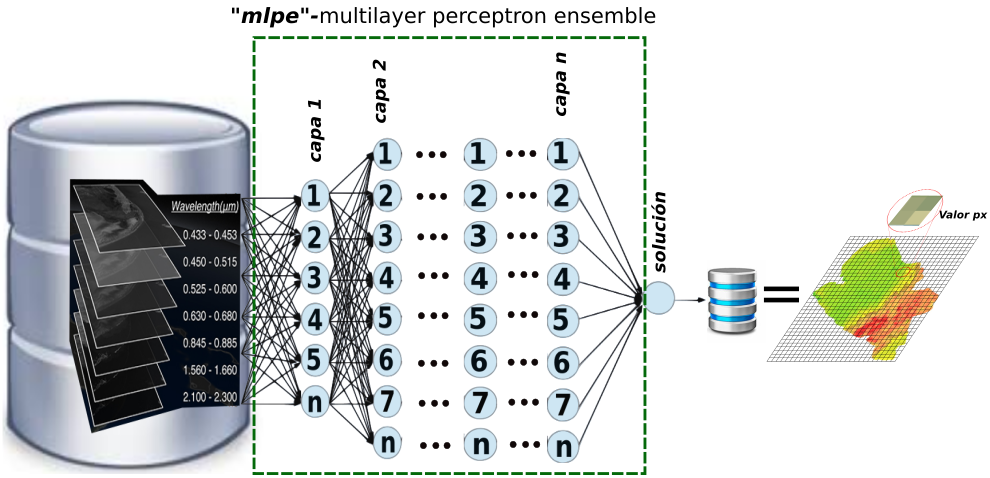
\includegraphics[scale=0.43]{pictures/mlpe.png}
  \caption{Proceso construcción serie de tiempo radiación solar a partir de imágenes satelitales LandSat y MODIS} 
  \label{fig:mlpe}
\end{figure}


\section{Mapas de Radiación Aplicando Interpolación Espacial}
 
La manera más adecuada de visualizar la información es mediante la creación de mapas de promedios mensuales, anuales y un promedio general 
de radiación solar sobre el departamento de Nariño. Una vez construida la serie de tiempo, se procede obtener agregados 
mensuales con el objetivo de establecer cual es el mes con más alta o baja radiación solar, el promedio anual es necesario para establecer como es la variación de la 
radiación solar en el transcurso del tiempo y el promedio general permite establecer la radiación solar promedio en Nariño para los 11 años de MODIS o 15 años de 
LandSat. Una vez obtenidos los agregados mensuales y anuales se desarrolló un script en R que permite implementar la interpolación espacial aplicando el método 
kriging mediante el uso de una grilla de 450x450m que indica la resolución del pixel para el mapa de radiación generado, adicionalmente se debe parametrizar 
el sistema de referencia de coordenadas estándar EPSG:3857 y formato GeoTiff para los mapas ver figuras~\ref{fig:g},~\ref{fig:agregadosm}y ~\ref{fig:agregadosa}; 
estos parámetros sirven para cualquier manejo cartográfico o manipulación de los mapas en un SIG.

\begin{figure}[htb]
  \centering 
  \subfigure[Mapa general de radiación solar MODIS]{\label{b1} 
  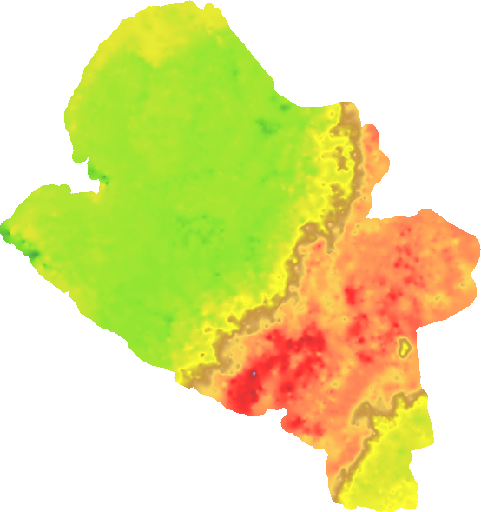
\includegraphics[scale=0.3]{pictures/mapM.png}}\hspace{10mm}
  \subfigure[Mapa general de radiación LandSat]{\label{b2} 
  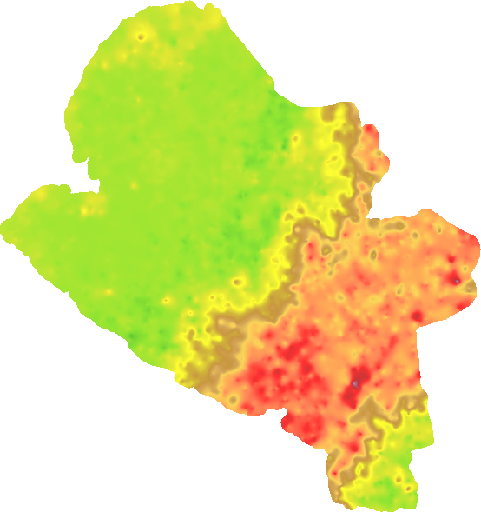
\includegraphics[scale=0.3]{pictures/mapL.png}} 
  \label{fig:g}
  \caption{Promedios de radiación solar}
\end{figure}

En terminos generales el mapa de radiación de MODIS tiene mayor número de muestras en comparación con los mapas de LandSat, pero se puede observar
similaridad en la imágenes al representar la estimación de radiación solar sobre el departamento de Nariño.

\begin{figure}[htb]
  \centering
  \subfigure[Mapas mensuales de radiación solar MODIS]{\label{b3} 
  \includegraphics[scale=0.3]{pictures/months.pdf}}\hspace{5mm}
  \subfigure[Mapa mensuales de radiación solar LandSat]{\label{b4} 
  \includegraphics[scale=0.25]{pictures/monthsL.pdf}}
  \label{fig:agregadosm}
  \caption{Promedios Mensuales}
\end{figure}

\begin{figure}[htb]
  \centering
  \subfigure[Mapas anuales de radiación solar MODIS (2005-2015)]{\label{b5} 
  \includegraphics[scale=0.29]{pictures/years.pdf}}\hspace{4mm}
  \subfigure[Mapas anuales de radiación solar LandSat (2000-2014)]{\label{b6} 
  \includegraphics[scale=0.27]{pictures/yearsL.pdf}}
  \label{fig:agregadosa}
  \caption{Promedios Anuales}
\end{figure}

Los mapas en formato GeoTiff son almacenados en BD para mayor simplicidad en el manejo de información y reportes, de forma complementaria son presentados en la 
plataforma GEOAlternar \footnote{\url{http://geoalternar.udenar.edu.co}} ver figura~\ref{fig:plataforma} permitiendo visualizar mapas, datos de promedios mensuales, 
datos de promedios anuales, descargar datos, generar reportes y buscar información de radiación solar, eólica, biomasa e hídrica presente en cualquier punto dentro 
del territorio Nariñense.
\begin{figure}[tbp]
  \centering 
  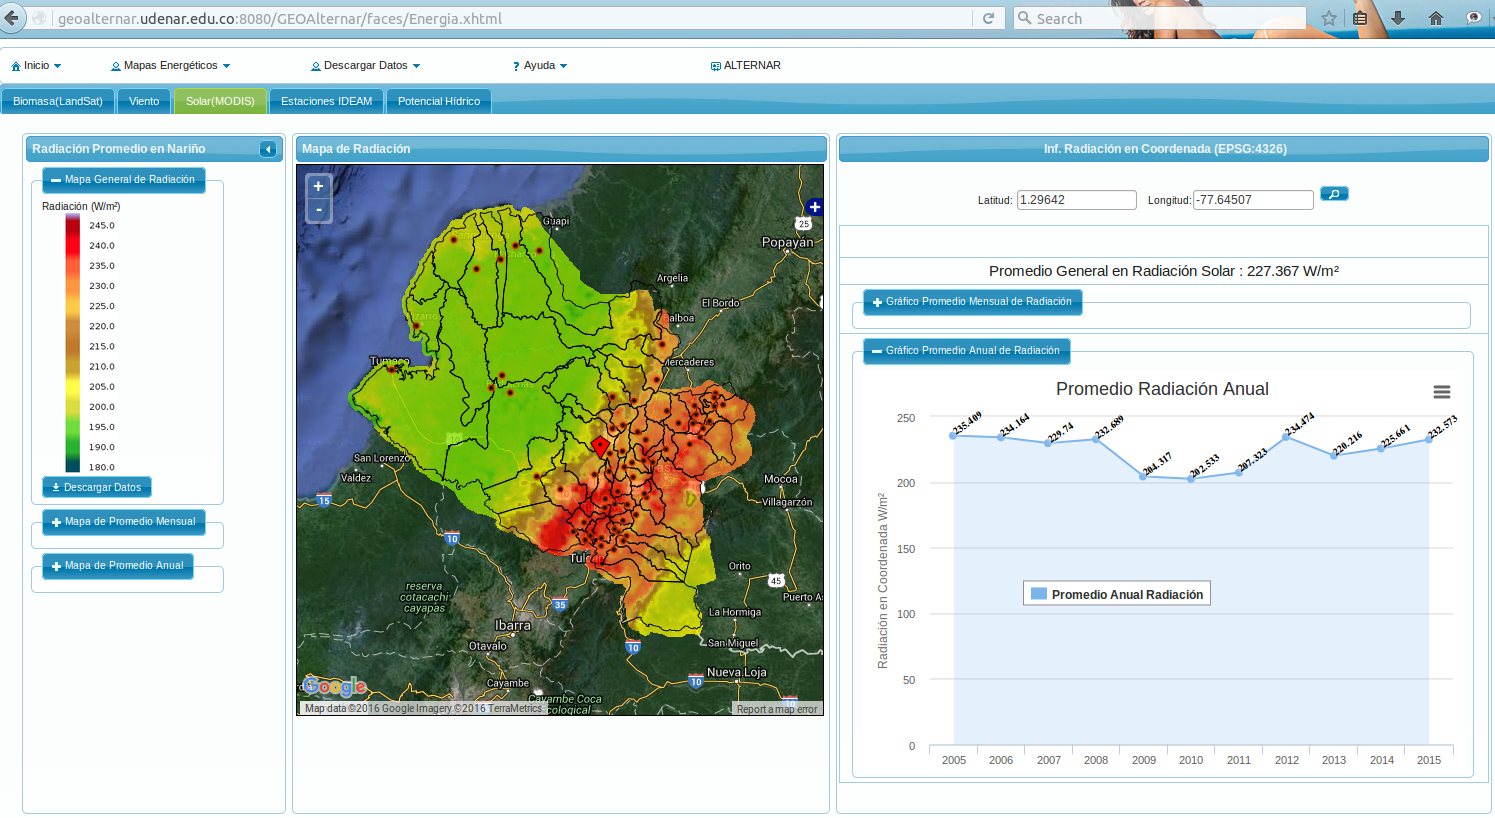
\includegraphics[scale=0.3]{pictures/plataforma.png}
  \caption{ Plataforma GEOAlternar- mapas energéticos del departamento de Nariño}
  \label{fig:plataforma}
\end{figure}

La gran ventaja de crear los mapas de radiación se ve reflejada en la fácil identificación de zonas con potencial de radiación solar, esta información es importante 
para futuras instalaciones de plantas energéticas a base de paneles solares o energía térmica, adicionalmente se puede contemplar el comportamiento mes a mes o año 
tras año de la radiación solar en una área específica.


\section{Detección de Patrones Secuenciales}

La detección de patrones secuenciales se las realizó utilizando la serie de tiempo construida anteriormente mediante los datos del sensor MODIS y el modelo mlpe.
Se aplicó un proceso de minería de datos a la serie de tiempo de radiación solar con el objetivo de extraer información de eventos frecuentes mediante 
la identificación de patrones secuenciales. Para este proceso se cuenta con las relaciones Irradiance y Datemodis ver figura~\ref{fig:insumos} con un historial 
de 11 años de datos que abarcan aproximadamente 340 millones de registros, también se realizó la selección de los 300 mejores puntos 
ver figura~\ref{fig:insumos} con mayor radiación solar dentro del departamento de Nariño, luego se sometió los registro 
histórico de radiación al algoritmo de LCM secuencial. 
\begin{figure*}[tb]
  \centering
  \subfigure[Mejores 300 puntos de radiación solar dentro del departamento de Nariño]{\label{b1} 
  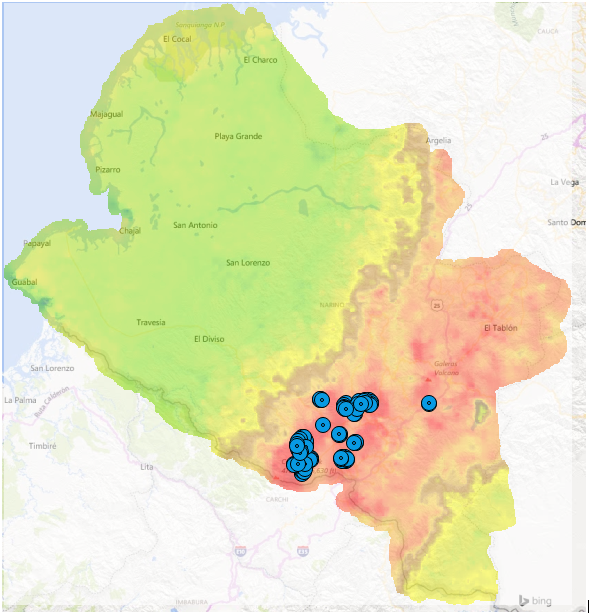
\includegraphics[scale=0.35]{pictures/300bp.png}}
  \subfigure[Relaciones para identificación de patrones secuenciales]{\label{b2} 
  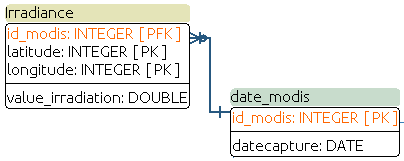
\includegraphics[scale=0.6]{pictures/bdpatterns.png}}
  \caption{Insumos para identificación de patrones secuenciales}
  \label{fig:insumos}
\end{figure*}
\newpage
La detección de patrones se realizó mediante el uso del algorítmo LCM secuencial\cite{uno2005lcm} el cual permite enumerar la frecuencia de acontecimientos 
presentes en una serie de tiempo; el algorítmo LCM secuencial cuenta con las funcionalidades necesarias para detección de patrones secuenciales por lo que 
es necesario establecer los parámetros para realiza la extracción de la información, para el proceso de minería se desarrolló un script en Python que permite 
ejecutar LCM secuencial y aplicarlo a la serie de tiempo de radiación solar utilizado los siguientes parámetros:
\begin{itemize}
 \item Serie de tiempo de muestra de radiación solar.
 \item Generación de 8 bines los cuales permiten discriminar la radiación como se muestra en la tabla~\ref{tabla:patrones}.
 \item Ventana de 30 dias para evaluar la ocurrencia de acontecimientos.
 \item Soporte de 90\%  para las transacciones.
\end{itemize}

\begin{table}[H]
\centering
\begin{tabular}{ >{\centering\arraybackslash}m{2cm} >{\centering\arraybackslash}m{5cm} >{\centering\arraybackslash}m{5cm}}
\hline
Bin & Rango radiación solar& Representación \\
\hline \hline
1 & (x<195.985) - 195.985 & 
\includegraphics[width=5mm]{pictures/suns/so1.png} \\
\hline
2 & 195.985 - 196.496 & 
\includegraphics[width=5mm]{pictures/suns/so2.png} \\
\hline
3 & 196.496 - 197.047 & 
\includegraphics[width=5mm]{pictures/suns/so3.png} \\
\hline
4 & 197.047 - 199.124 & 
\includegraphics[width=5mm]{pictures/suns/so4.png} \\
\hline
5 & 199.124 - 205.954 & 
\includegraphics[width=5mm]{pictures/suns/so5.png} \\
\hline
6 & 205.954 - 228.426 & 
\includegraphics[width=5mm]{pictures/suns/so6.png} \\
\hline
7 & 228.426 - 233.534 & 
\includegraphics[width=5mm]{pictures/suns/so7.png} \\
\hline
8 & 233.534 - (x>233.534) & 
\includegraphics[width=5mm]{pictures/suns/so8.png} \\
\hline
\end{tabular}
\caption{Bines utilizados en la detección y representación de patrones secuenciales.}
\label{tabla:patrones}
\end{table}

Se implementó el algorítmo incluyendo los parámetros correspondientes, el pseudo-código base propuesto se contempla en Algorítmo ~\ref{alg:patt}.

\begin{algorithm}
  \renewcommand{\algorithmicrequire}{\textbf{Input:}}
  \renewcommand{\algorithmicensure}{\textbf{Output:}}
  \caption{Identificación de Patrones Secuenciales}
  \label{alg:patt}
  \algsetup{indent=2em}
  \footnotesize
  \begin{algorithmic}[1]
    \REQUIRE {BD Seie de Tiempo Radiación}
    \ENSURE {Patrones de Radiación Solar}
    \STATE $ListaPatrones \leftarrow \emptyset$
    \FOR { $SerieTiempoMuestraReflectancia_{lat,lon} \in$ BD Serie de Tiempo Radiación}
      \STATE $Soporte \leftarrow $90\%
      \STATE $Bines \leftarrow $[Tabla ~\ref{tabla:patrones}]
      \FOR {$Ventana \in SerieTiempoMReflectancia_{lat,lon}$}
	  \STATE {Patron $\leftarrow$ Aplicar $LCM\_seq(_{MReflectancia(_{lat,lon}), Bines,Soporte})$  \tiny{ LCM Algorithm \cite{uno2005lcm}}}
	  \STATE {FP $\leftarrow Patron_{Frecuente}$ }
	  \STATE {DP $\leftarrow Patron_{Diferente}$ }
	  \STATE {TP $\leftarrow Patron_{Tamaño}$ }
	\ENDFOR
      \STATE $ListaPatrones \leftarrow FP,DP,TP$ 
      \STATE $ALmacenar Patron DB$ 
    \ENDFOR
  \end{algorithmic}
\end{algorithm}

Los resultados obtenidos son almacenados en BD ver figura~\ref{fig:bdp} para posteriormente proceder al análisis y visualización. Tal y como muestra la figura~\ref{fig:bdp}
se creó la relación ``patrones por día'' que presenta 8 atributos donde los más relevantes para identificar patrones son detallados a continuación.

\texttt{\noindent
\phantom{x}\hspace{5ex}$latitude-longitude\to $\footnotesize Ubicación geográfica en el sistema de coordenadas EPSG:3857 \\
\phantom{x}\hspace{6ex}$pattern\to $ \footnotesize Representa la detección de un conjunto de bines del la tabla ~\ref{tabla:patrones}. \\
\phantom{x}\hspace{6ex}$len\_pattern\to $\footnotesize Indica el número consecutivo de dias de la ocurrencia de un evento.\\
\phantom{x}\hspace{6ex}$frecuency\to $\footnotesize Indica la frecuencia del patrón detectado.\\
\phantom{x}\hspace{6ex}$solar\to $\footnotesize Representa el conjunto de bines en el rango de la escala solar~\ref{tabla:patrones}.\\
\phantom{x}\hspace{6ex}$diff\_solar\to $\footnotesize Registra los tipos de bines que hay en el patrón.\\
}

Para la representación visual de los patrones detectados en los 300 mejores puntos de radiación, se desarrolló un script para generar un archivo kml que permite
visualizar la ubicación geográfica, dias presentes y frecuencia del patrón como lo muestra la figura~\ref{fig:visualizarpatron}, el archivo es desplegado sobre la plataforma google-earth.

\begin{figure}[htbp]
  \centering 
  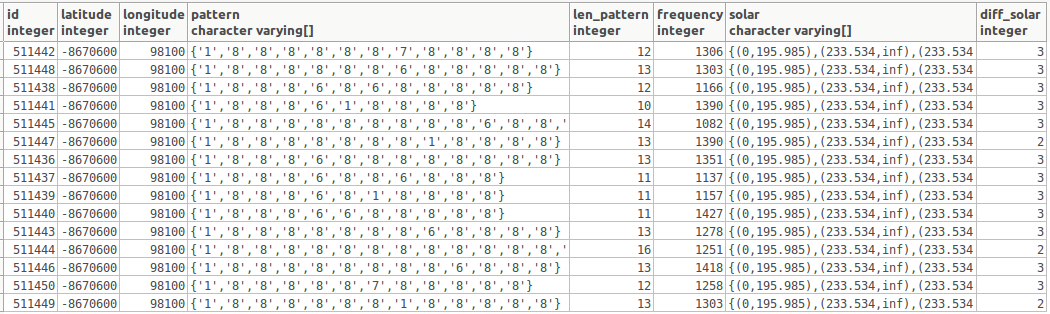
\includegraphics[scale=0.40]{pictures/bdp.png}
  \caption{Base de datos resultado de aplicación LCM secuencial}
  \label{fig:bdp}
  \centering
  \subfigure[Ubicación geográfica de los patrones de radiación en departamento de Nariño]{\label{b1} 
  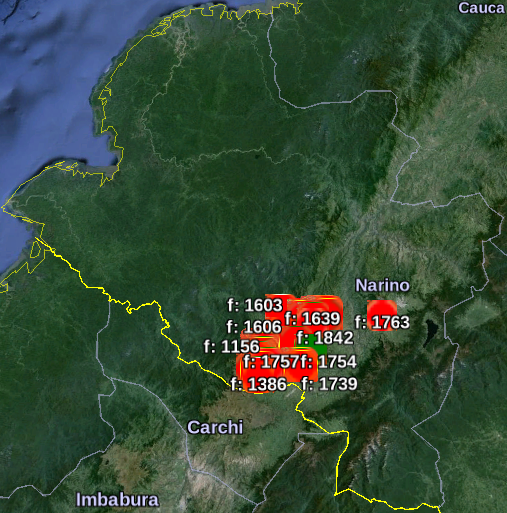
\includegraphics[scale=0.27]{pictures/ugp.png}}
  \subfigure[Acercamiento a zona con patrones de radiación solar]{\label{b2} 
  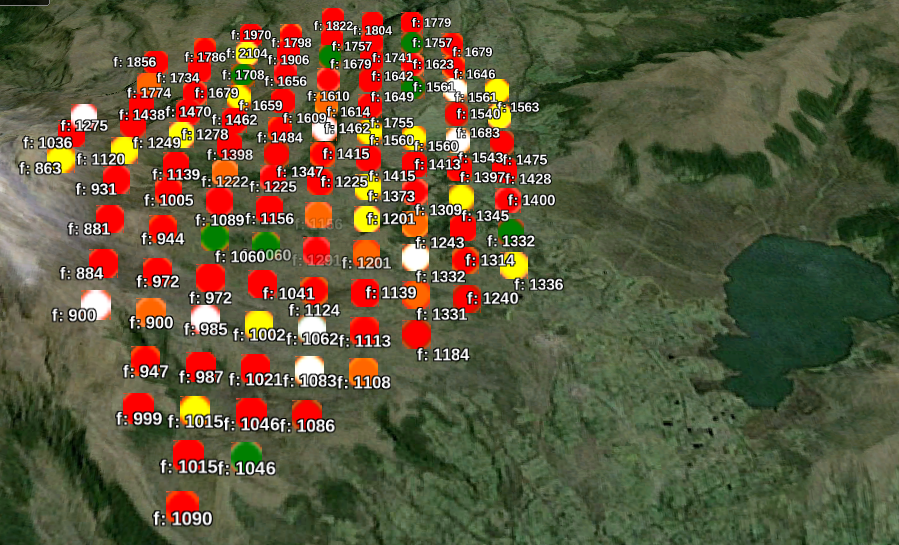
\includegraphics[scale=0.25]{pictures/apg.png}}
  \subfigure[Detalle de patrón de radiación solar]{\label{b3} 
  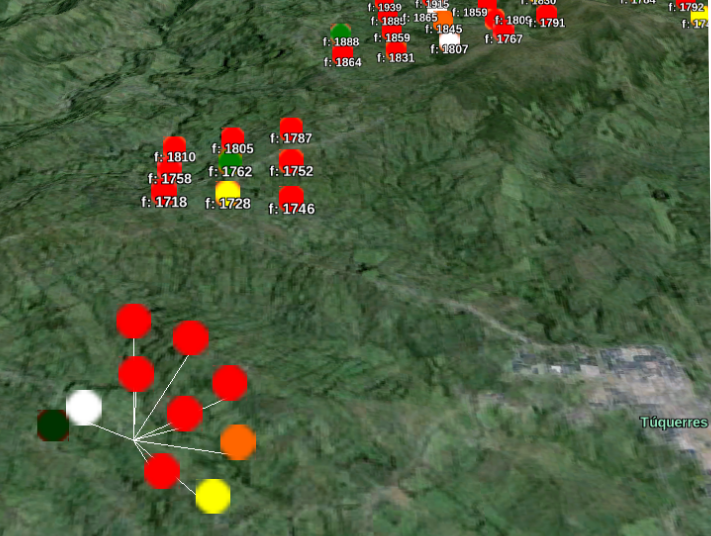
\includegraphics[scale=0.25]{pictures/pdg.png}}
  \caption{Visualización de patrones de radiación solar}
  \label{fig:visualizarpatron}
\end{figure}

Los patrones detectados anteriormente permiten establecer un periodo de de tiempo con presencia de radiación solar constante, en este periodo se puede aprovechar 
al máximo las plantas solares debido a que se puede garantizar una óptima radiación solar por un numero determinado de dias.
\newpage

\section{Comportamiento de Nubes}

El comportamiento de las nubes está estrechamente ligado a la producción de energía a base de paneles de radiación solar
o energía térmica, por este motivo fué necesario construir un registro histórico referente a la presencia de nubes, 
este registro permite evidenciar la presencia de aerosoles sobre el departamento de Nariño, haciendo
posible la identificación de la presencia de de nubosidad en una zona con potencial de radiación solar. La identificación de nubes se realizó 
mediante filtros aplicados a las muestras de reflectancia, el filtro se implemento teniendo en cuenta el tratamiento y las recomendaciones necesarias 
que se deben dar a las bandas de la imagen satelital\cite{modisweb}\cite{bandMODISspecification}\cite{cea2005mejoras}.

Para identificar el comportamiento de las nubes se utilizó el registro histórico con el objetivo de establecer la probabilidad 
para la presencia de nubes en una zona determinada. Como primera medida se construyó una BD donde se almacena la 
probabilidad de la presencia de nubes en un punto determinado para construir la BD fué necesario realizar un conteo de los dias
del mes en los que se presentó nubes en cada punto dentro del departamento de Nariño, posteriormente se agrupo mensual y anualmente para calcular 
la probabilidad y establecer un promedio para la presencia de nubes en un punto determinado dentro del departamento de Nariño.

Los promedios mensuales permiten establecer como es el comportamiento de las nubes en el tiempo para un
punto específico dentro del territorio Nariñense, la información de nubosidad tiene varios campos de aplicación, con estos datos se hace posible 
prever la presencia  nubosidad sobre plantas de energía solar en un periodo determinado y tomar medidas adicionales para mitigar los efectos, 
por ejemplo, si se logra determinar en que zonas hay periodos de abundante radiación pero también existe una época donde se presenta gran nubosidad;
esta información permite contrarrestar los periodos de baja radiación mediante el uso de generadores de energía con fuentes alternativas como eólica, 
hídrica o biomasa.

A continuación se realiza un análisis del comportamiento de nubes en un punto especifico dentro del departamento de Nariñofiguras~\ref{fig:mc}, este análisis se
lo puede realizar en cualquier zona que se encuentre dentro del territorio nariñense debido a que el las muestras de nubes detectadas también son interpoladas 
aplicando el método de kriging para el todo el departamento.
\begin{figure}[htb]
  \centering 
  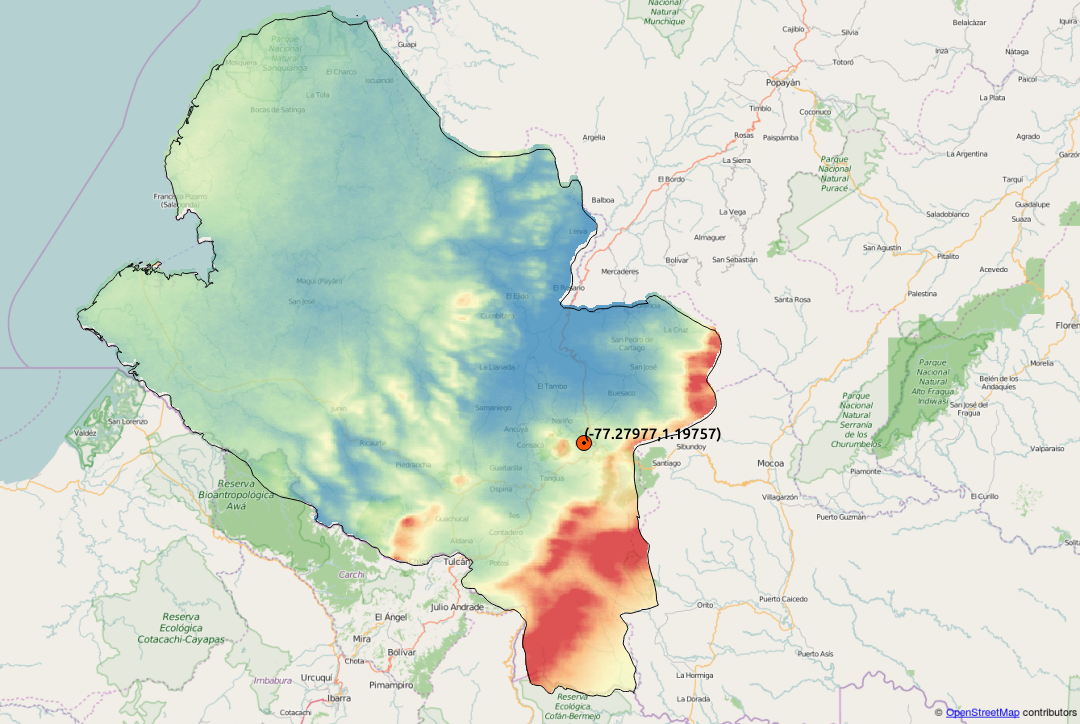
\includegraphics[scale=0.45]{pictures/mc.png}
  \caption{Comportamiento mensual de nubes en un punto específico}
  \label{fig:mc}
\end{figure}

En las figuras~\ref{fig:nubesmes} y ~\ref{fig:nubesy} se logra observar los registros en la coordenada (-77.27977,1.19757); como lo muestra el el 
gráfico ~\ref{fig:nubesmes} se observa que en 5 meses el porcentaje de nubosidad supera el 20\% permitiendo establecer que 7 dias del mes el territorio 
se encuentra nublado por lo que se hace necesario tener una alternativa energética diferente para solventar la posible reducción de energía a base de 
paneles solares, por otro lado el comportamiento de las nubes en el transcurso de los 11 años de información es regulado debido a que se encuentra alrededor 
del 20\% lo que indica que en promedio 75 dias del año esta zona se encuentra cubierta de nubes.

\begin{figure}[htb]
  \centering 
  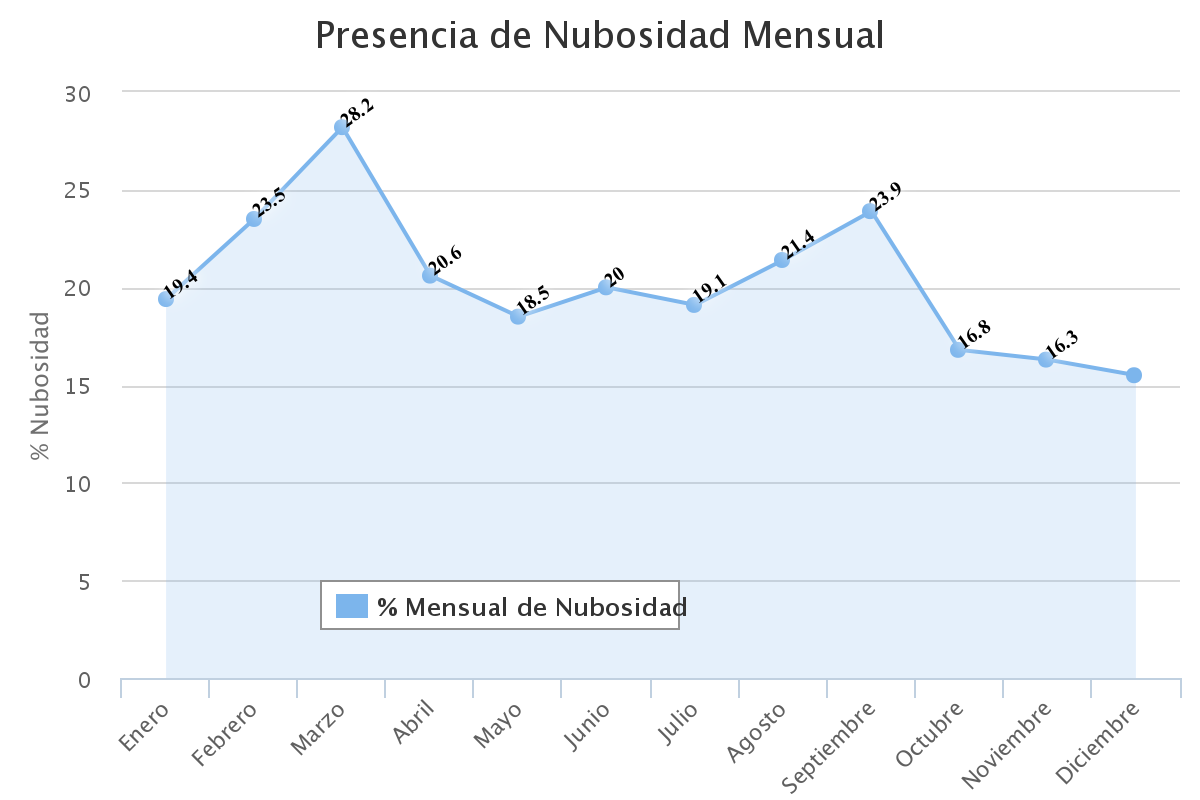
\includegraphics[scale=0.25]{pictures/nm.png}
  \caption{Comportamiento mensual de nubes en un punto específico}
  \label{fig:nubesmes}
\end{figure}
\begin{figure}[htb]
  \centering 
  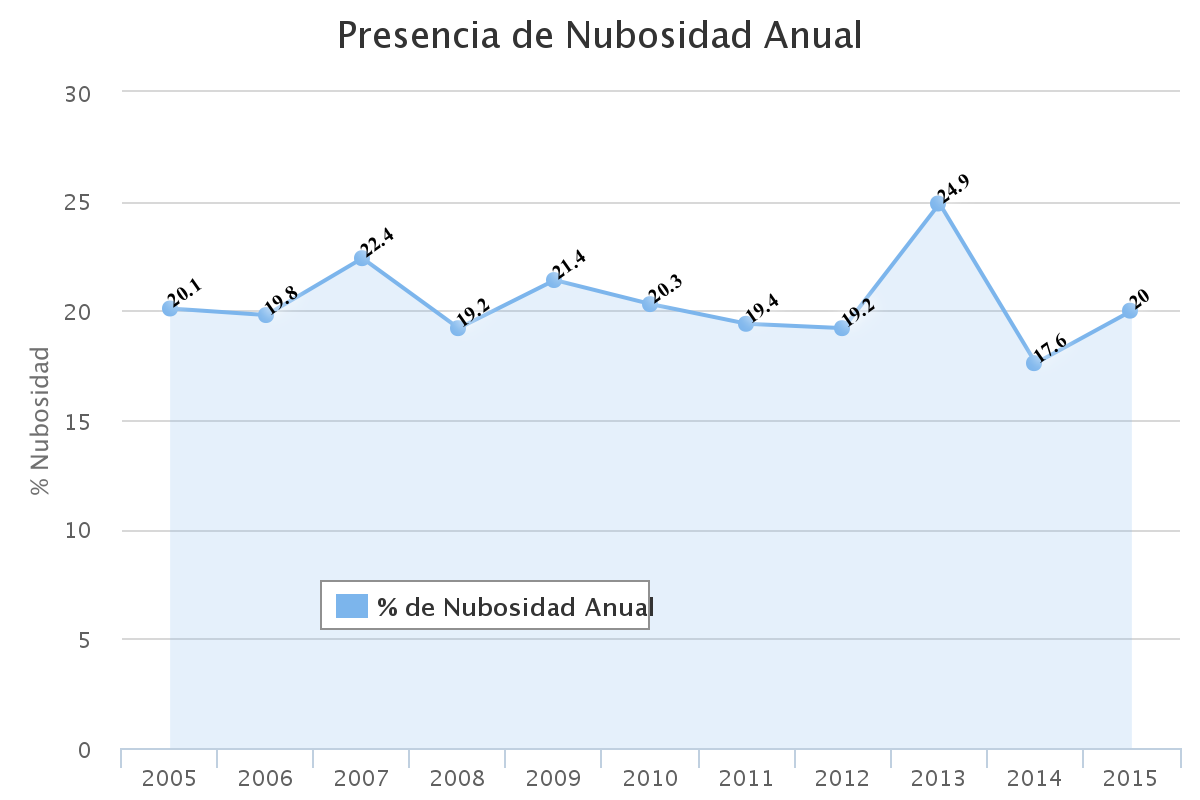
\includegraphics[scale=0.25]{pictures/ny.png}
  \caption{Comportamiento Anual de nubes en un punto específico}
  \label{fig:nubesy}
\end{figure}